\documentclass[a4paper,12pt]{book}
\usepackage[margin=0.7in,nomarginpar]{geometry}
\usepackage[utf8]{inputenc}
\usepackage{graphicx}
\usepackage{mathtools}
\usepackage{amsfonts}
\usepackage{hyperref}
\usepackage{tabularx}
\usepackage{array}
\usepackage{xcolor}
\usepackage{circuitikz}
\usepackage{polynom}
\usepackage{wrapfig}
\usepackage[italian]{babel}
\usepackage{float}
\restylefloat{table}
\usepackage{mathtools}
\graphicspath{ {./images/} }

\DeclarePairedDelimiter\ceil{\lceil}{\rceil}
\DeclarePairedDelimiter\floor{\lfloor}{\rfloor}

\addtolength{\topmargin}{.2in}
\addtolength{\textheight}{-.3in}

\newcommand{\overbar}[1]{\mkern 1.5mu\overline{\mkern-1.5mu#1\mkern-1.5mu}\mkern 1.5mu}

\def\C{\mathbb{C}}
\def\N{\mathbb{N}}
\def\Q{\mathbb{Q}}
\def\R{\mathbb{R}}
\def\Z{\mathbb{Z}}

\begin{document}

\author{Alessandro Cheli - Prof. Marco Danelutto}
\title{Appunti di Architettura degli Elaboratori}
\date{A.A 2019-2020}

\frontmatter
\maketitle
\tableofcontents

\mainmatter
\part{}
\chapter{Introduzione al Corso}

\begin{itemize}
	\item{\textbf{Logica Booleana}}
	\item{\textbf{Aritmetica Binaria}}
	\item{\textbf{Reti Logiche}}
	\item{\textbf{Microarchitettura e Assembler ARM v7 e v8}}
	\item{\textbf{Gestione della memoria}}
	\item{\textbf{I/O}}
\end{itemize}


\begin{defn}
	\textbf{Strumenti Software} \\

	A differenza degli A.A passati utilizzeremo Verilog e Assembler ARM.
	Utilizzeremo \textbf{iverilog} come compilatore Verilog e \textbf{gtkwave} come tool grafico. Un ambiente di sviluppo Verilog completo che vedremo è \textbf{Quartus}.
	Per la seconda parte del corso, Assembler ARM, useremo la \textbf{toolchain GNU}, in particolare:
	
	
	\subparagraph{Se non hai una macchina ARM:}
	\begin{itemize}
		\item{cross-compiler per compilare}
		\item{QEMU per una macchina virtuale ARM}
		\item{gdb per debugging}
	\end{itemize}
	
	\subparagraph{Se hai una macchina ARM come un Raspberry Pi:}
	\begin{itemize}
		\item{Toolchain GNU per compilare}
		\item{Cavo Ethernet}
		\item{Server SSH sulla macchina ARM per accesso remoto}
	\end{itemize}
\end{defn}

\begin{note}
	\textbf{Storia degli Elaboratori}\\
	
	\begin{figure}
		\centering
		\caption{Sinclair ZX80}
		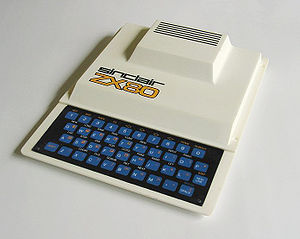
\includegraphics[width=0.5\textwidth]{ZX80}
	\end{figure}
	
	Nei corsi di Architettura degli Elaboratori negli anni 80 i processori studiati erano: il 6502 (8 bit, processore del computer Apple II, noto per essere stato costruito nel garage di Steve Jobs e Wozniak), Z80, processore a 16 bit del famoso computer ZX80 e l'Intel 8088. Tali processori raggiungevano al massimo una velocità di clock (detto molto a grandi linee, operazioni al secondo) dell'ordine di meno di una decina di MHz (Mega Hertz, milioni). I processori odierni raggiungono
	cicli di clock sull'ordine dei GHz (Giga Hertz, miliardi). Nel corso degli anni fino ad oggi, l'evoluzione dei processori ha seguito la \textbf{legge di Moore}. La "legge" spiega che ogni 18 mesi la potenza dei processori in commercio raddoppia, perché la densità dei transistor contenuti all'interno aumenta. Negli ultimi decenni abbiamo  miglioramenti architetturali come super pipeline e super scalari, ciò ha permesso di introdurre processori \textbf{multicore}, ovvero che contengono più "nuclei" interni (detti core) che elaborano le istruzioni dei processi in esecuzione in parallelo.
	Ad oggi il numero di core in uno smartphone raggiunge anche gli 8 core, mentre in processori per server sono stati raggiunti numeri di core anche intorno ai 64. I processori odierni utilizzano core a 64 bit, con architettura X86\_64 per Desktop o ARM per dispositivi mobili.
	Un componente fondamentale dell'evoluzione degli elaboratori è stato anche lo sviluppo dei processori grafici (GPU) con i quali ad oggi è possibile riprodurre grafica su schermo, ambienti tridimensionali molto complessi (videogiochi) o sfruttare la loro capacità di parallelizzazione per l'uso di reti neurali nell'intelligenza artificiale.
	
	Osserveremo i calcolatori a diversi livelli di \textbf{astrazione}
	
	I livelli di astrazione sono:
	\begin{itemize}
		\item Applicazioni utente
		\item Sistema Operativo
		\item Architettura (ASM, ad es. x86 o ARM)
		\item Microarchitettura
		\item Logica
		\item Circuiti digitali
		\item Device
		\item Fisica
	\end{itemize}
	
	Ogni livello si appoggia sul livello inferiore, ovvero è costruito sui componenti offerti dal livello inferiore. Dei principi fondamentali sono: \textbf{gerarchi, modularità e regolarità}
	
	La modularità è fondamentale per avere moduli organizzati gerarchicamente, autonomi ed indipendenti.
\end{note}



\begin{defn}
	\textbf{Set di Istruzioni}

	Distinguiamo due set di istruzioni dei processori, \textbf{CISC} e \textbf{RISC}. Gli acronimi sono rispettivamente \textbf{Complex Instruction Set Computer} e \textbf{Reduced Instruction Set Computer}, RISC contiene i processori ARM, che studieremo in dettaglio, mentre CISC comprende i processori più comuni nei desktop (X86 e X86\_64)
\end{defn}


\chapter{Rappresentazioni Numeriche e Testuali}

\section{Aritmetica Binaria}

I calcolatori utilizzano valori discreti (differenze di potenziale) fra 0 e 1 per rappresentare valori numerici. Viene detta Aritmetica Binaria l'aritmetica con i numeri rappresentati in base 2.

Siamo abituati a ragionare in base 10, ad esempio il numero 413 in base 10 è 
\[ 104 = 10^2 \cdot 1 + 10^1 \cdot 0 + 10^0 \cdot 4 \]

Lo stesso numero rappresentato in base 2 (codice binario) è

\[ 104_{10} = 01101000_2 = 2^7 \cdot 0 + 2^6 \cdot 1 + 2^5 \cdot 1 + 2^4 \cdot 0 + 2^3 \cdot 1 + 2^2 \cdot 0 + 2^1 \cdot 0 + 2^0 \cdot 0 \]

Un numero binario di 8 cifre è detto \textbf{byte}, un numero di 4 cifre è detto \textbf{nibble}. Una \textbf{parola} (\textbf{word}) è la quantità minima su cui viene rappresentato un intero in un calcolatore. Ad oggi le parole dei calcolatori sono 64 bit, alcuni calcolatori datati hanno parole da 32 bit.

La somma nell'aritmetica binaria è definita normalmente per i numeri positivi. Nei calcolatori i numeri hanno una dimensione finita (numero di bit) che indica il numero di cifre binarie con le quali è possibile rappresentare un numero. I positivi binari rappresentano numeri fino a $ 2^{N}-1 $ dove $ N $ è il numero di cifre.

Per rappresentare i numeri negativi si utilizza il metodo \textbf{segno-magnitudo} dove il bit più a sinistra rappresenta il segno (0 se il numero è positivo e 1 se è negativo). Il problema del metodo segno-magnitudo è che non rispetta la somma aritmetica. Può rappresentare numeri da $ [-2^{N-1}, +2^{N-1} ] $

Un metodo migliore per rappresentare i numeri negativi è il \textbf{complemento a due}. Nel complemento a due la cifra più a sinistra rappresenta sempre $ 2^{N-1} $ ma \textbf{negativo}. Il resto delle cifre sono positive e vengono sommate alla prima cifra negativa. Questo metodo rispetta la somma aritmetica. Per moltiplicare un numero per $ -1 $ si invertono le cifre binarie e si aggiunge 1 al numero. È possibile anche la sottrazione sommando un numero positivo ad uno negativo.

La somma fra due cifre può essere costruita con reti logiche. Il risultato della somma $ A + B = A \oplus B $ (operatore XOR) mentre il riporto della somma = $ A \land B $ (operatore AND)

\begin{figure}
	\centering
	\caption{Gate XOR}
	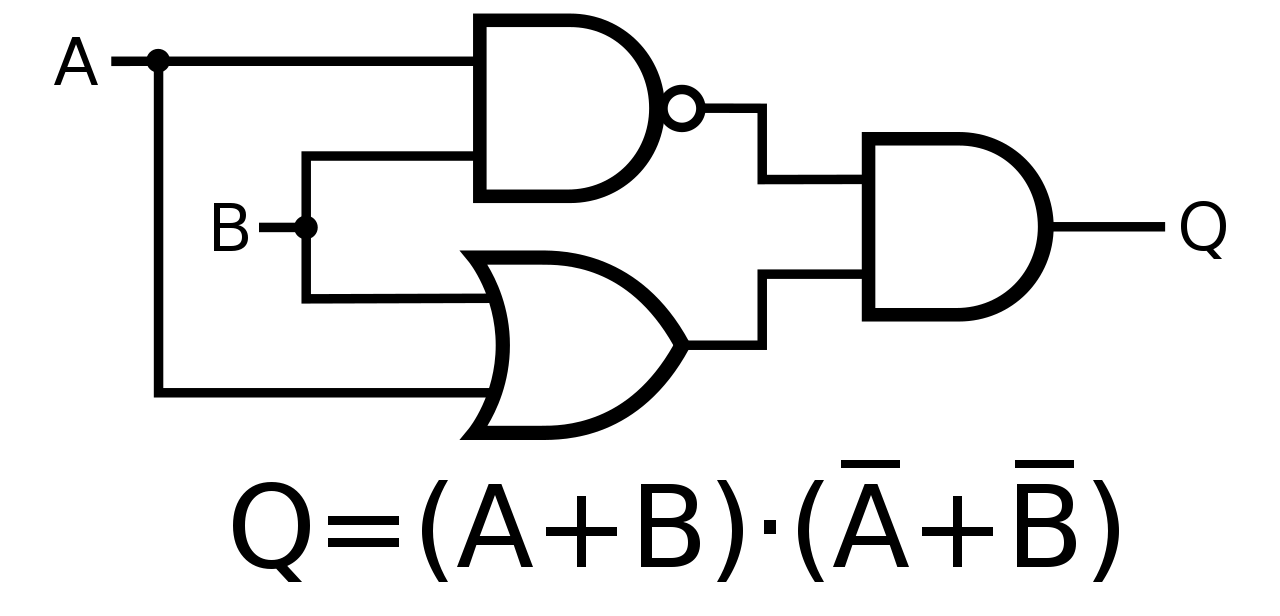
\includegraphics[width=\textwidth/2]{xor}
\end{figure}

\section{Esadecimale} 

I numeri esadecimali sono numeri in base 16. Siccome non bastano le cifre decimali per rappresentare i numeri maggiori di 9 si usano le prime lettere dell'alfabeto.
Una cifra esadecimale rappresenta un nibble (4 bit).

\section{Numeri in virgola mobile}

I numeri in virgola mobile si rappresentano con lo standard EEE 754 che definisce come si rappresentano i numeri in virgola mobile a singola precisione e doppia precisione (32 e 64 bit)

I bit del numero vengono divisi in 3 parti. Il primo bit denota il segno, la seconda parte rappresenta l'esponente e la terza parte si denota mantissa. L'esponente esprime dove la virgola verrà posizionata, come nella notazione scientifica di una calcolatrice l'esponente rappresenta $ 10^{n} $ dove $ n $ è l'esponente. La mantissa è un numero di base moltiplicato per $ 10^0 $, e viene successivamente moltiplicato per l'esponente.
L'esponente può essere sia positivo che negativo.

\begin{figure}
	\caption{Standard IEEE 754 a 32 bit}
	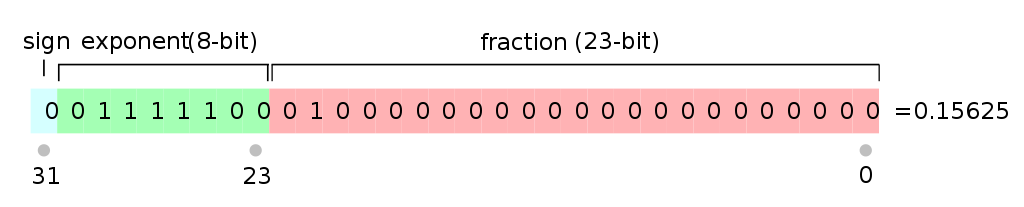
\includegraphics[width=\textwidth]{eee_floating_32}
\end{figure}

Nello standard a 32 bit la sezione esponente ha 8 bit di lunghezza. Un numero ad 8 bit può rappresentare numeri da 0 a 255, per ottenere gli esponenti negativi nello standard dei numeri a virgola mobile il numero a 8 bit rappresenta invece numeri da -127 a +128

\begin{figure}
	\caption{IEEE 754 a 64 bit}
	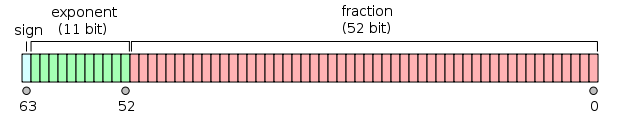
\includegraphics[width=\textwidth]{eee_floating_64}
\end{figure}

\paragraph{Somma dei numeri a virgola mobile}

Per sommare i numeri a virgola mobile il primo passo è allineare le mantisse, significa osservare gli esponenti e spostarli fino a che le cifre non sono sommabili in colonna.
Il secondo passo consiste nel sommare e il terzo passo nel normalizzare la somma. Nei processori la somma floating point viene eseguita in dei moduli appositi che in input ricevono due o più numeri floating point ed eseguono in dei sotto-moduli i tre passaggi della somma in un tempo $ 1/3 t $ dove $ t $ è il tempo totale per eseguire una somma. I tre passaggi della somma possono essere sequenzializzati così che una volta che ogni sotto-modulo ha completato il passo, può ricevere subito l'input successivo (la somma di due numeri FP impiegherà $ t + 1/3 $ invece che $ 2t $)

\paragraph{Estensioni vettoriali}
Alcuni processori permettono di eseguire operazioni contemporaneamente su un registro dividendolo in sottoregistri più piccoli. 

\section{Codifica ASCII}
La codifica ASCII è una tabella di codifica di caratteri testuali con interi da 0 a 255 (8 bit). La codifica ASCII estesa è a 16 bit e comprende diversi caratteri non latini.

\begin{figure}
	\caption{Tabella ASCII}
	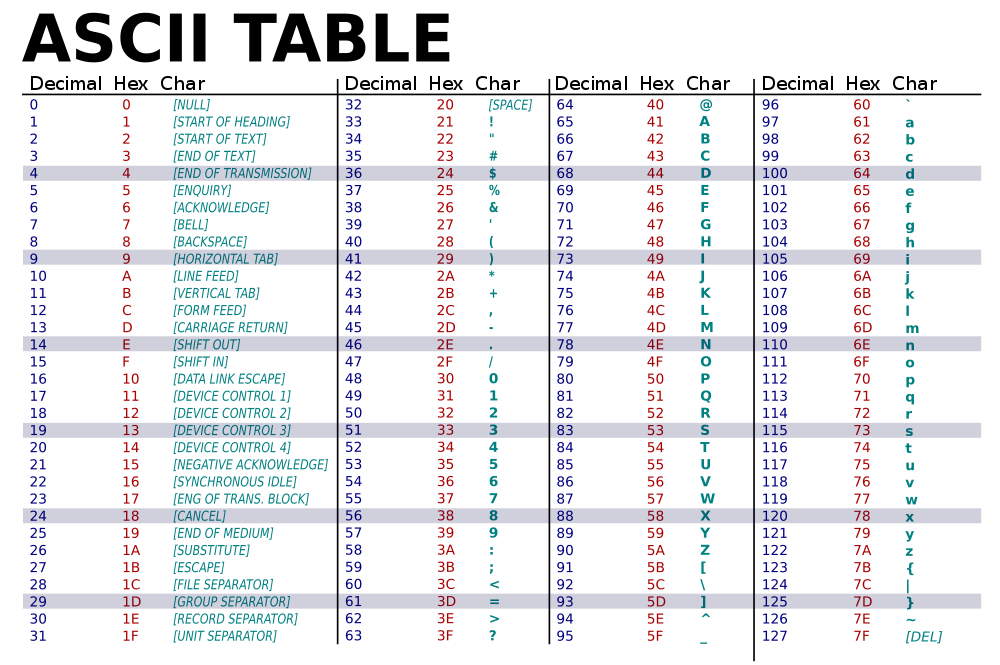
\includegraphics[width=\textwidth]{ascii}
\end{figure}

\section{Porte Logiche e Algebra di Boole}

I circuiti digitali vengono realizzati utilizzando componenti chiamati \textbf{porte logiche}. Sono realizzate con componenti fisici come transistor e resistenze, ma nella progettazione dei circuiti digitali le porte logiche vengono schematizzate con i simboli riportati nella Figura 3.1 per semplificare la progettazione \textbf{astraendo} il livello di complessità della circuiteria analogica.
Solamente con la porta NAND si possono realizzare tutte le altre porte (NAND è funzionalmente completo), ma le porte in generale si costruiscono singolarmente con componenti appositi. Esse implementano la \textbf{logica booleana} che conseguentemente permette di realizzare operazioni di \textbf{aritmetica binaria} per costruire unità di calcolo in componenti elettronici e processori.

\begin{wrapfigure}{r}{0.6\textwidth}
	\begin{center}
		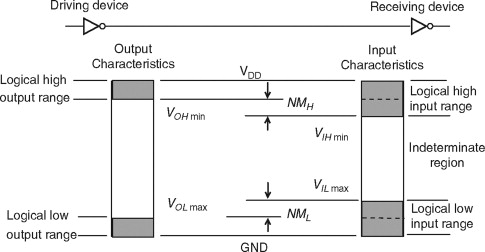
\includegraphics[width=0.58\textwidth]{noisemargin}
	\end{center}
	\caption{Margine di rumore nei circuiti digitali}	
\end{wrapfigure}


I componenti elettronici molto piccoli sono sensibili al \textbf{rumore}, per ovviare al problema i valori discreti (0 e 1) nei circuiti digitali non seguono un cambiamento istantaneo di differenza di potenziale (voltaggio), ma ammettono un margine per ridurre i problemi causati dal rumore.


I componenti (transistor) con cui si costruiscono porte logiche e circuiti sono realizzati con materiali semiconduttori, che possono essere di diversi tipi. Vedremo il tipo NMOS. Un transistor è composto da materiali come gallio e silicio.

\begin{wrapfigure}{r}{0.7\textwidth}
	\begin{center}
		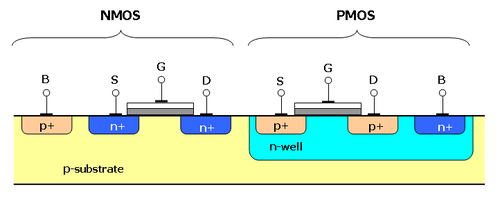
\includegraphics[width=0.68\textwidth]{cmos}
	\end{center}
	\caption{Transistor NMOS}
\end{wrapfigure}


\begin{figure}
	\centering
	\caption{Tabella delle porte logiche comuni}
	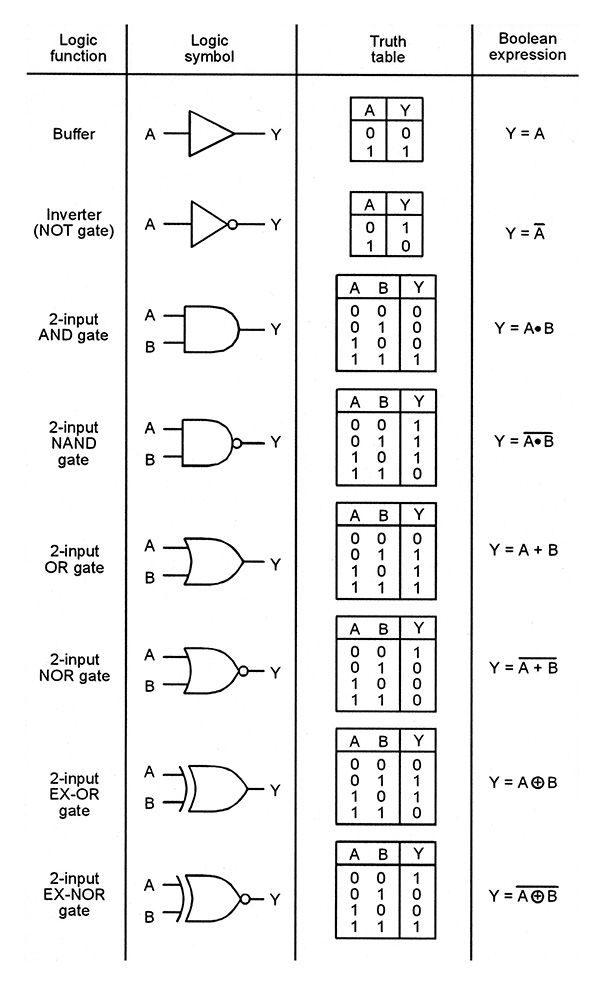
\includegraphics[width=\textwidth,height=\textheight]{logicgates}
\end{figure}

\begin{figure}
	\centering
	\caption{Porta NOT con transistor PMOS e NMOS}
	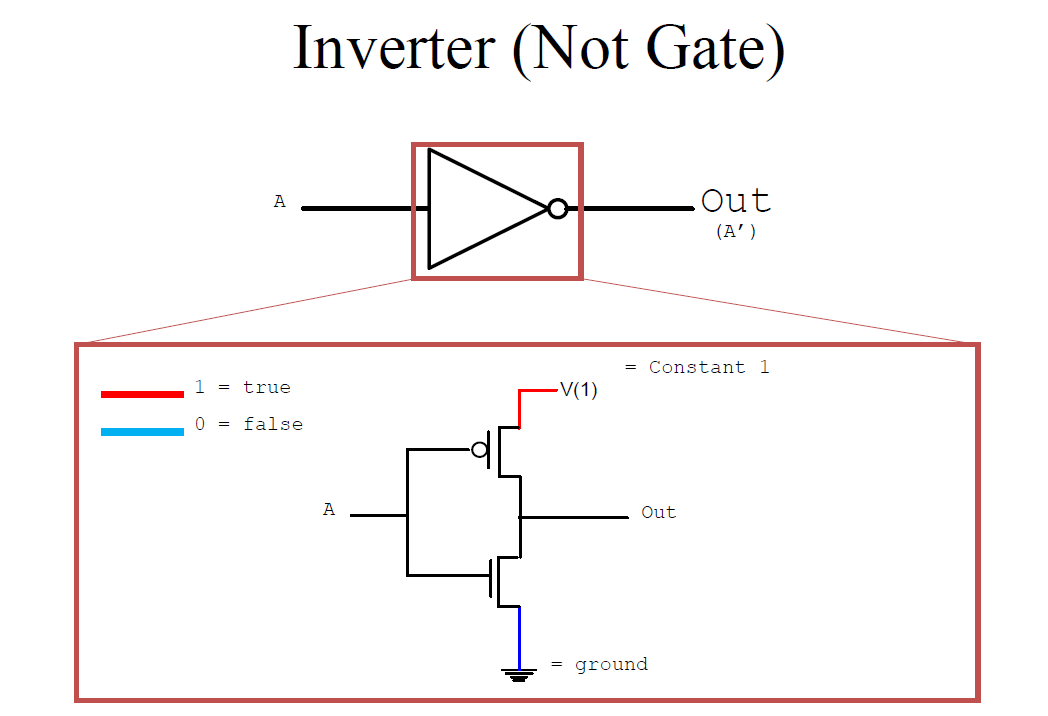
\includegraphics[width=\textwidth]{notgatetransistor}
\end{figure}

\begin{figure}
	\centering
	\caption{Transistor NMOS e PMOS}
	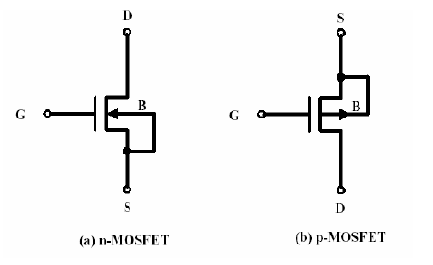
\includegraphics[width=0.6\textwidth]{NMOS-and-PMOS}
\end{figure}

\clearpage

\subsection{Algebra di Boole}


\begin{figure}[H]
	\centering
	
\includegraphics[width=0.48\textwidth]{sommadiprodotti-gate}
	\caption{Conversione di $ z $ da formula booleana a circuito logico}
\end{figure}

\begin{table}[H]
	\centering
	\caption{Notazione usata per l'Algebra di Boole}
	\label{tab:notazione-booleana}
	\begin{tabular}{|l|l|l|}
		\hline
		Funzione & Notazione Usata & Notazione Logica \\ 
		NOT(A)   & $\overbar{A}$   & $\lnot A$        \\ 
		AND(A,B) & $A \cdot B$     & $A \land B$      \\ 
		OR(A,B)  & $A + B$         & $A \lor B$       \\ \hline
	\end{tabular}
\end{table}

Prendiamo ad esempio un espressione booleana in forma canonica in \textbf{somma di prodotti}:
\[ z = \overbar{A}\overbar{B}\overbar{C} + \overbar{A}\overbar{B}C + \overbar{A}BC + A\overbar{B}C + ABC \]


\begin{table}[H]
	\centering
	\caption{Tabella di verità di $ z $}
	\label{tab:z-truth}
	\begin{tabular}{|l|l|l|l|}
		\hline
		A & B & C & z \\ \hline
		0                       & 0                      & 0 & 1 \\  
		0                       & 0                      & 1 & 1 \\ 
		0                       & 1                      & 0 & 0 \\ 
		0                       & 1                      & 1 & 1 \\ 
		1                       & 0                      & 0 & 0 \\ 
		1                       & 0                      & 1 & 1 \\  
		1                       & 1                      & 0 & 0 \\ 
		1                       & 1                      & 1 & 1 \\ \hline
	\end{tabular}
\end{table}




$ z $ si può anche esprimere come prodotto di somme: $ z = (A+\overbar{B}+C)(\overbar{A}BC)(\overbar{A}\overbar{B}C) $


\subsection{Teoremi dell'Algebra Booleana}
Breve ripasso dei teoremi della Logica Booleana.
\paragraph{Elemento Identità di prodotto e somma}
\[ A \cdot 1 = A \iff A \land T \equiv A\]
\[ A + 0 = 0 \iff A \lor F \equiv A\]
\paragraph{Elemento assorbente}
\[ A \cdot 0 = 0 \iff A \land F \equiv F \]
\[ A + 1 = 1 \iff A \lor T \equiv T \]
\paragraph{Idempotenza}
\[ A \cdot A = A \iff A \land A \equiv A \]
\[ A + A = A \iff A \lor A \equiv A \]
\paragraph{Complemento}
\[ A \cdot \overbar{A} = 0 \iff A \land \lnot A \equiv F \]
\[ A + \overbar{A} = 1 \iff A \lor \lnot A \equiv T \]
\paragraph{Commutatività}
\[ A + B = B + A \]
\[ A \cdot B = B \cdot A \]
\paragraph{Associatività}
\[ (A \cdot B) \cdot C = A \cdot (B \cdot C) \]
\[ (A + B) + C = A + (B + C) \]
\paragraph{Distributività}
\[ (A \cdot B) + C = (A+C) \cdot (B+C) \]
\[ (A+B) \cdot C = AC + BC \]
\paragraph{DeMorgan}
\[ \overbar{(A + B)} = \overbar{A} \cdot \overbar{B} \iff \lnot(A \lor B )\equiv \lnot A \land \lnot B \]
\[ \overbar{(A \cdot B)} = \overbar{A} + \overbar{B} \iff \lnot(A \land B )\equiv \lnot A \lor \lnot B \]

\paragraph{Esempio}
Semplifichiamo la formula booleana $ z = \overbar{A}\overbar{B}\overbar{C} + \overbar{A}\overbar{B}C + \overbar{A}BC + A\overbar{B}C + ABC $

\begin{align}
\begin{cases}
\overbar{A}\overbar{B}\overbar{C} + \overbar{A}\overbar{B}C \equiv \overbar{A}\overbar{B}(\overbar{C}+C) \equiv \overbar{A}\overbar{B} \\ 
A\overbar{B}C + ABC \equiv AC(\overbar{B}+B) \equiv AC
\end{cases} \\
\implies z = \overbar{A}\overbar{B} + \overbar{A}BC + AC
\end{align}

Le leggi della logica Booleana ci permettono di semplificare molto i componenti realizzati con porte logiche.

\subsection{Mappe di Karnaugh}

Una mappa di Karnaugh o K-Map è un metodo di semplificare un espressione booleana. I valori sono trasferiti da una tabella di verità ad una mappa bidimensionale:

Approfondisci su \href{https://en.wikipedia.org/wiki/Karnaugh_map}{Wikipedia}

Prendiamo una formula a quattro variabili $ f(A,B,C,D) $, una mappa di Karnaugh può essere:
\begin{table}[H]
	\centering
	\caption{Tabella di verità della mappa di Karnaugh di $f$}
	\label{tab:karnaugh}
	\begin{tabular}{lllll}
		AB\textbackslash{}CD    & 00                     & 01                     & 11                     & 10                     \\ \cline{2-5} 
		\multicolumn{1}{l|}{00} & \multicolumn{1}{l|}{1} & \multicolumn{1}{l|}{1} & \multicolumn{1}{l|}{1} & \multicolumn{1}{l|}{1} \\ \cline{2-5} 
		\multicolumn{1}{l|}{01} & \multicolumn{1}{l|}{1} & \multicolumn{1}{l|}{1} & \multicolumn{1}{l|}{0} & \multicolumn{1}{l|}{0} \\ \cline{2-5} 
		\multicolumn{1}{l|}{11} & \multicolumn{1}{l|}{0} & \multicolumn{1}{l|}{1} & \multicolumn{1}{l|}{0} & \multicolumn{1}{l|}{0} \\ \cline{2-5} 
		\multicolumn{1}{l|}{10} & \multicolumn{1}{l|}{0} & \multicolumn{1}{l|}{0} & \multicolumn{1}{l|}{1} & \multicolumn{1}{l|}{1} \\ \cline{2-5} 
	\end{tabular}
\end{table}

Facciamo ad esempio la mappa di Karnaugh di $ z = f(A,B,C) $ vista nella sezione precedente:

\begin{table}[H]
	\centering
	\caption{Tabella di verità della mappa di Karnaugh di $z$}
	\label{tab:karnaugh}
	\begin{tabular}{lllll}
		A\textbackslash{}BC    & 00                     & 01                     & 11                     & 10                     \\ \cline{2-5} 
		\multicolumn{1}{l|}{0} & \multicolumn{1}{l|}{1} & \multicolumn{1}{l|}{1} & \multicolumn{1}{l|}{1} & \multicolumn{1}{l|}{0} \\ \cline{2-5} 
		\multicolumn{1}{l|}{1} & \multicolumn{1}{l|}{0} & \multicolumn{1}{l|}{1} & \multicolumn{1}{l|}{1} & \multicolumn{1}{l|}{0} \\ \cline{2-5} 
	\end{tabular}
\end{table}

Possiamo riconoscere un'implicante nella seconda e terza colonna che corrisponde esattamente a C. Osserviamo un'altra implicante nella prima riga, prima e seconda colonna che corrisponde esattamente a $ \overbar{A}\overbar{B} $. Possiamo poi sommare le implicanti per ottenere una formula equivalente a quella di partenza, ciò implica che $ z =  \overbar{A}\overbar{B} + C $


\subsection{Circuito con più output}
Se abbiamo una tabella di verità di un circuito con $ n $ input e $ 2^n $ righe, con più output $ z_1, \dots, z_k $, gli output si suddividono in $ k $ tabelle con un solo output ($ z_k $) e $ 2^n $ righe di input.

\subsection{Operatori a più ingressi}
Gli operatori a più ingressi AND, OR, etc..., se presentano più di due ingressi si rappresentano con una rete logica che sfrutta la proprietà associativa degli operatori logici. Ciò comporta un limite massimo di ingressi perché viene introdotto un ritardo di stabilizzazione determinato e piccolo.
Ad esempio, un AND a 4 ingressi sarà rappresentato come $ z = x_1 \cdot x_2 \cdot x_3 \cdot x_4 = (x_1 \cdot x_2 ) \cdot (x_3 \cdot x_4)  $
Perciò gli operatori associativi a più ingressi si rappresentano come un albero k-ario di porte logiche. Il numero di livelli di porte sarà $ log_k(n) $ dove $ k $ è l'arietà delle singole porte ed è $ n $ il numero di ingressi nel circuito.

% TODO figura albero di AND con 8 input. 


\chapter{Porte Logiche e Algebra di Boole}

I circuiti digitali vengono realizzati utilizzando componenti chiamati \textbf{porte logiche}. Sono realizzate con componenti fisici come transistor e resistenze, ma nella progettazione dei circuiti digitali le porte logiche vengono schematizzate con i simboli riportati nella Figura 3.1 per semplificare la progettazione \textbf{astraendo} il livello di complessità della circuiteria analogica.
Solamente con la porta NAND si possono realizzare tutte le altre porte (NAND è funzionalmente completo), ma le porte in generale si costruiscono singolarmente con componenti appositi. Esse implementano la \textbf{logica booleana} che conseguentemente permette di realizzare operazioni di \textbf{aritmetica binaria} per costruire unità di calcolo in componenti elettronici e processori.

\begin{wrapfigure}{r}{0.6\textwidth}
	\begin{center}
		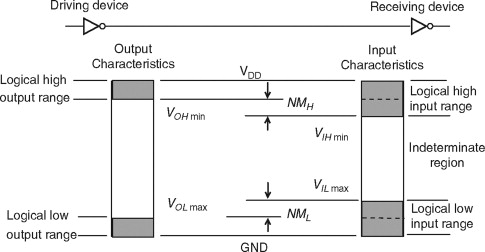
\includegraphics[width=0.58\textwidth]{noisemargin}
	\end{center}
	\caption{Margine di rumore nei circuiti digitali}	
\end{wrapfigure}


I componenti elettronici molto piccoli sono sensibili al \textbf{rumore}, per ovviare al problema i valori discreti (0 e 1) nei circuiti digitali non seguono un cambiamento istantaneo di differenza di potenziale (voltaggio), ma ammettono un margine per ridurre i problemi causati dal rumore.


I componenti (transistor) con cui si costruiscono porte logiche e circuiti sono realizzati con materiali semiconduttori, che possono essere di diversi tipi. Vedremo il tipo NMOS. Un transistor è composto da materiali come gallio e silicio.

\begin{wrapfigure}{r}{0.7\textwidth}
	\begin{center}
		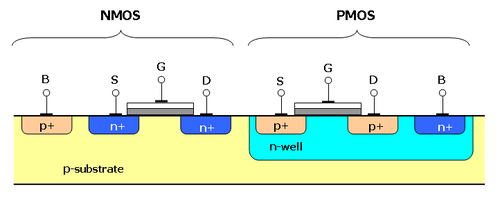
\includegraphics[width=0.68\textwidth]{cmos}
	\end{center}
	\caption{Transistor NMOS}
\end{wrapfigure}


\begin{figure}
	\centering
	\caption{Tabella delle porte logiche comuni}
	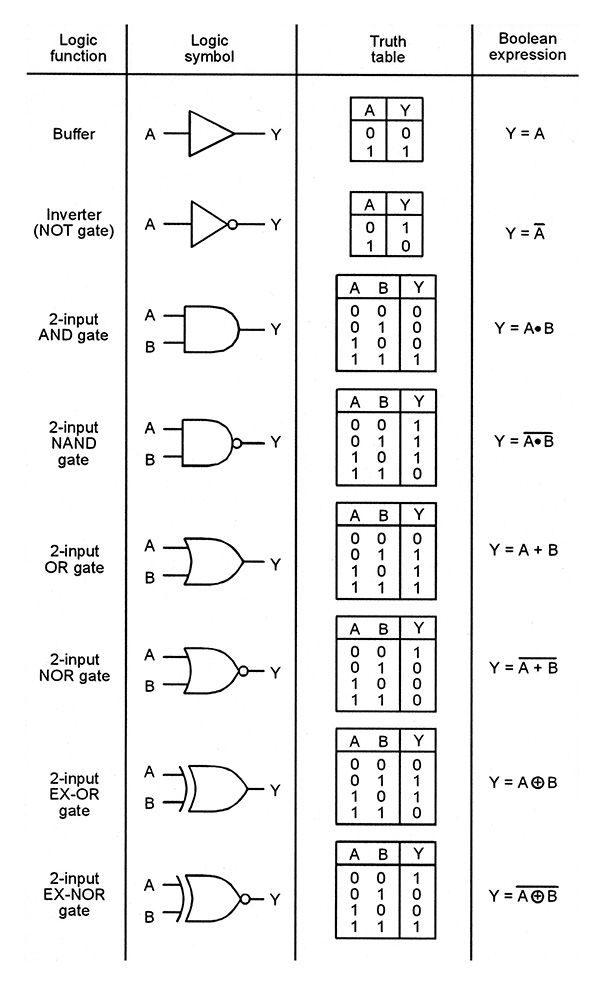
\includegraphics[width=\textwidth,height=\textheight]{logicgates}
\end{figure}

\begin{figure}
	\centering
	\caption{Porta NOT con transistor PMOS e NMOS}
	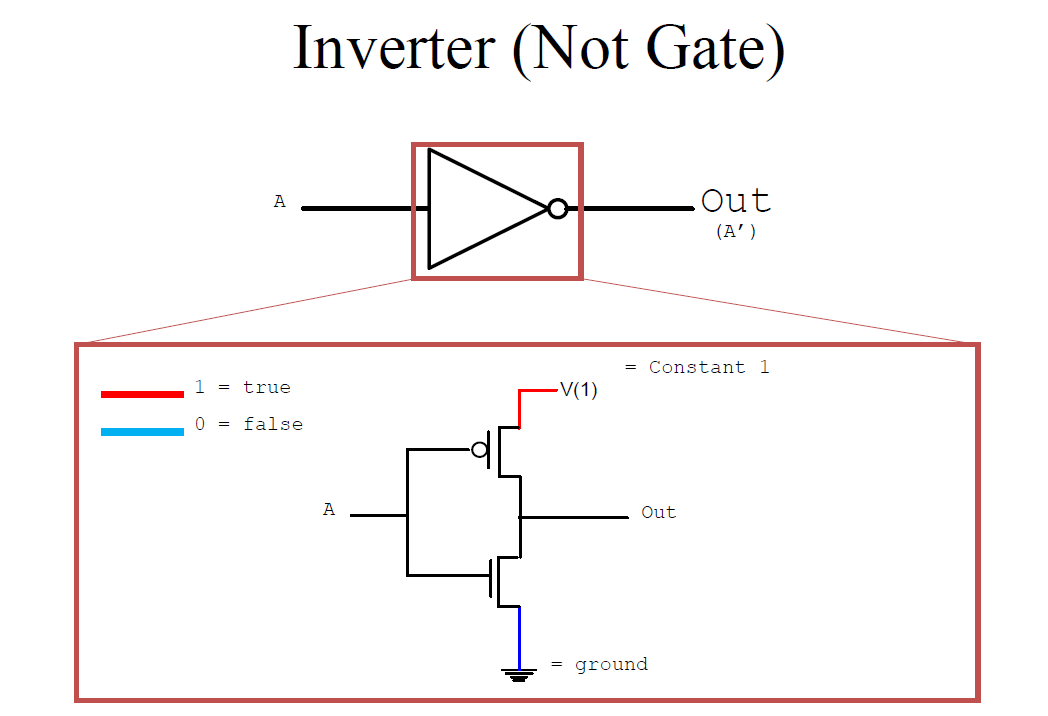
\includegraphics[width=\textwidth]{notgatetransistor}
\end{figure}

\begin{figure}
	\centering
	\caption{Transistor NMOS e PMOS}
	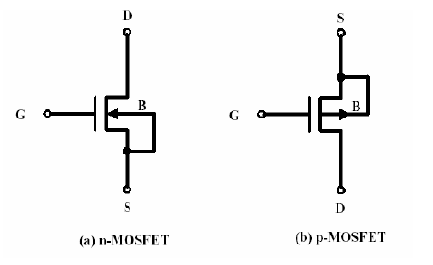
\includegraphics[width=0.6\textwidth]{NMOS-and-PMOS}
\end{figure}

\clearpage

% TODO porta logica NOT con MOS


\section{Algebra di Boole}

\begin{table}[H]
	\centering
	\caption{Notazione usata per l'Algebra di Boole}
	\label{tab:notazione-booleana}
	\begin{tabular}{|l|l|l|}
		\hline
		Funzione & Notazione Usata & Notazione Logica \\ 
		NOT(A)   & $\overbar{A}$   & $\lnot A$        \\ 
		AND(A,B) & $A \cdot B$     & $A \land B$      \\ 
		OR(A,B)  & $A + B$         & $A \lor B$       \\ \hline
	\end{tabular}
\end{table}

La forma canonica di espressioni booleane in \textbf{somma di prodotti} è:
\[ z = \overbar{A}\overbar{B}\overbar{C} + \overbar{A}\overbar{B}C + \overbar{A}BC + A\overbar{B}C + ABC \]

\begin{table}[H]
	\centering
	\caption{Tabella di verità di $ z $}
	\label{tab:z-truth}
	\begin{tabular}{|l|l|l|l|}
		\hline
		A & B & C & z \\ \hline
		0                       & 0                      & 0 & 1 \\  
		0                       & 0                      & 1 & 1 \\ 
		0                       & 1                      & 0 & 0 \\ 
		0                       & 1                      & 1 & 1 \\ 
		1                       & 0                      & 0 & 0 \\ 
		1                       & 0                      & 1 & 1 \\  
		1                       & 1                      & 0 & 0 \\ 
		1                       & 1                      & 1 & 1 \\ \hline
	\end{tabular}
\end{table}

$ z $ si può anche esprimere come prodotto di somme: $ z = (A+\overbar{B}+C)(\overbar{A}BC)(\overbar{A}\overbar{B}C) $

% TODO conversione da forma canonica somma di prodotti a circuito 4.3

\section{Teoremi dell'Algebra Booleana}
Breve ripasso dei teoremi della Logica Booleana.
\paragraph{Elemento Identità di prodotto e somma}
\[ A \cdot 1 = A \iff A \land T \equiv A\]
\[ A + 0 = 0 \iff A \lor F \equiv A\]
\paragraph{Elemento assorbente}
\[ A \cdot 0 = 0 \iff A \land F \equiv F \]
\[ A + 1 = 1 \iff A \lor T \equiv T \]
\paragraph{Idempotenza}
\[ A \cdot A = A \iff A \land A \equiv A \]
\[ A + A = A \iff A \lor A \equiv A \]
\paragraph{Complemento}
\[ A \cdot \overbar{A} = 0 \iff A \land \lnot A \equiv F \]
\[ A + \overbar{A} = 1 \iff A \lor \lnot A \equiv T \]
\paragraph{Commutatività}
\[ A + B = B + A \]
\[ A \cdot B = B \cdot A \]
\paragraph{Associatività}
\[ (A \cdot B) \cdot C = A \cdot (B \cdot C) \]
\[ (A + B) + C = A + (B + C) \]
\paragraph{Distributività}
\[ (A \cdot B) + C = (A+C) \cdot (B+C) \]
\[ (A+B) \cdot C = AC + BC \]
\paragraph{DeMorgan}
\[ \overbar{(A + B)} = \overbar{A} \cdot \overbar{B} \iff \lnot(A \lor B )\equiv \lnot A \land \lnot B \]
\[ \overbar{(A \cdot B)} = \overbar{A} + \overbar{B} \iff \lnot(A \land B )\equiv \lnot A \lor \lnot B \]

\paragraph{Esempio}
Semplifichiamo la formula booleana $ z = \overbar{A}\overbar{B}\overbar{C} + \overbar{A}\overbar{B}C + \overbar{A}BC + A\overbar{B}C + ABC $

\begin{align}
\begin{cases}
\overbar{A}\overbar{B}\overbar{C} + \overbar{A}\overbar{B}C \equiv \overbar{A}\overbar{B}(\overbar{C}+C) \equiv \overbar{A}\overbar{B} \\ 
A\overbar{B}C + ABC \equiv AC(\overbar{B}+B) \equiv AC
\end{cases} \\
\implies z = \overbar{A}\overbar{B} + \overbar{A}BC + AC
\end{align}

Le leggi della logica Booleana ci permettono di semplificare molto i componenti realizzati con porte logiche.

\section{Mappe di Karnaugh}

% TODO cos'è una mappa di Karnaugh

Prendiamo una formula a quattro variabili $ f(A,B,C,D) $, una mappa di Karnaugh può essere:
\begin{table}[H]
	\centering
	\caption{Tabella di verità della mappa di Karnaugh di $f$}
	\label{tab:karnaugh}
	\begin{tabular}{lllll}
		AB\textbackslash{}CD    & 00                     & 01                     & 11                     & 10                     \\ \cline{2-5} 
		\multicolumn{1}{l|}{00} & \multicolumn{1}{l|}{1} & \multicolumn{1}{l|}{1} & \multicolumn{1}{l|}{1} & \multicolumn{1}{l|}{1} \\ \cline{2-5} 
		\multicolumn{1}{l|}{01} & \multicolumn{1}{l|}{1} & \multicolumn{1}{l|}{1} & \multicolumn{1}{l|}{0} & \multicolumn{1}{l|}{0} \\ \cline{2-5} 
		\multicolumn{1}{l|}{11} & \multicolumn{1}{l|}{0} & \multicolumn{1}{l|}{1} & \multicolumn{1}{l|}{0} & \multicolumn{1}{l|}{0} \\ \cline{2-5} 
		\multicolumn{1}{l|}{10} & \multicolumn{1}{l|}{0} & \multicolumn{1}{l|}{0} & \multicolumn{1}{l|}{1} & \multicolumn{1}{l|}{1} \\ \cline{2-5} 
	\end{tabular}
\end{table}

Facciamo ad esempio la mappa di Karnaugh di $ z = f(A,B,C) $ vista nella sezione precedente:

\begin{table}[H]
	\centering
	\caption{Tabella di verità della mappa di Karnaugh di $z$}
	\label{tab:karnaugh}
	\begin{tabular}{lllll}
		A\textbackslash{}BC    & 00                     & 01                     & 11                     & 10                     \\ \cline{2-5} 
		\multicolumn{1}{l|}{0} & \multicolumn{1}{l|}{1} & \multicolumn{1}{l|}{1} & \multicolumn{1}{l|}{1} & \multicolumn{1}{l|}{0} \\ \cline{2-5} 
		\multicolumn{1}{l|}{1} & \multicolumn{1}{l|}{0} & \multicolumn{1}{l|}{1} & \multicolumn{1}{l|}{1} & \multicolumn{1}{l|}{0} \\ \cline{2-5} 
	\end{tabular}
\end{table}

Possiamo riconoscere un'implicante nella seconda e terza colonna che corrisponde esattamente a C. Osserviamo un'altra implicante nella prima riga, prima e seconda colonna che corrisponde esattamente a $ \overbar{A}\overbar{B} $. Possiamo poi sommare le implicanti per ottenere una formula equivalente a quella di partenza, ciò implica che $ z =  \overbar{A}\overbar{B} + C $


\subsection{Circuito con più output}
Se abbiamo una tabella di verità di un circuito con $ n $ input e $ 2^n $ righe, con più output $ z_1, \dots, z_k $
\chapter{Reti Sequenziali, Verilog e RTL}

Gli RTL, o Register Transfer Language, permettono di descrivere cosa succede a livello di circuito fra registri. Vengono utilizzati per descrivere l'hardware. Vedremo il linguaggio \textbf{Verilog}. Gli RTL permettono di descrivere e comporre dei moduli. Il libro di testo propone il dialetto \textbf{System Verilog} che mette a disposizione due metodi per descrivere i moduli. Un metodo è il metodo \textit{constructive}, noi vedremo il metodo \textit{behavioral} dove ad esempio un Multiplexer da 2 vie 1 bit è descritto da:
\begin{lstlisting}[style={verilog}]
	z = (ic == 0 ? x : y)
\end{lstlisting}

Verilog è un linguaggio compilato. Un file System Verilog compilato produce una traccia di esecuzione e un eseguibile che simula il comportamento dei moduli. Viene detta \textbf{simulazione}.

Un programma Verilog può anche essere dato in input a un programma detto \textbf{synthetizer}, che produce una \textbf{netlist}, ovvero una lista dei componenti e dei collegamenti per realizzare il modulo fisicamente. Un altro modo per realizzare la sintesi è utilizzare un \textbf{FPGA}, o Field-programmable gate array. Un FPGA è un circuito integrato composto da una matrice di celle, e una singola cella può:
\begin{enumerate}
	\item Eseguire una funzione booleana di 3-5 ingressi con 1 uscita 
	\item Implementare un bit di memoria
	\item Routing
\end{enumerate} 

Un FPGA moderno comprende, oltre a delle celle, delle righe che contengono diversi componenti come delle ALU.

\begin{figure}[H]
	\centering
	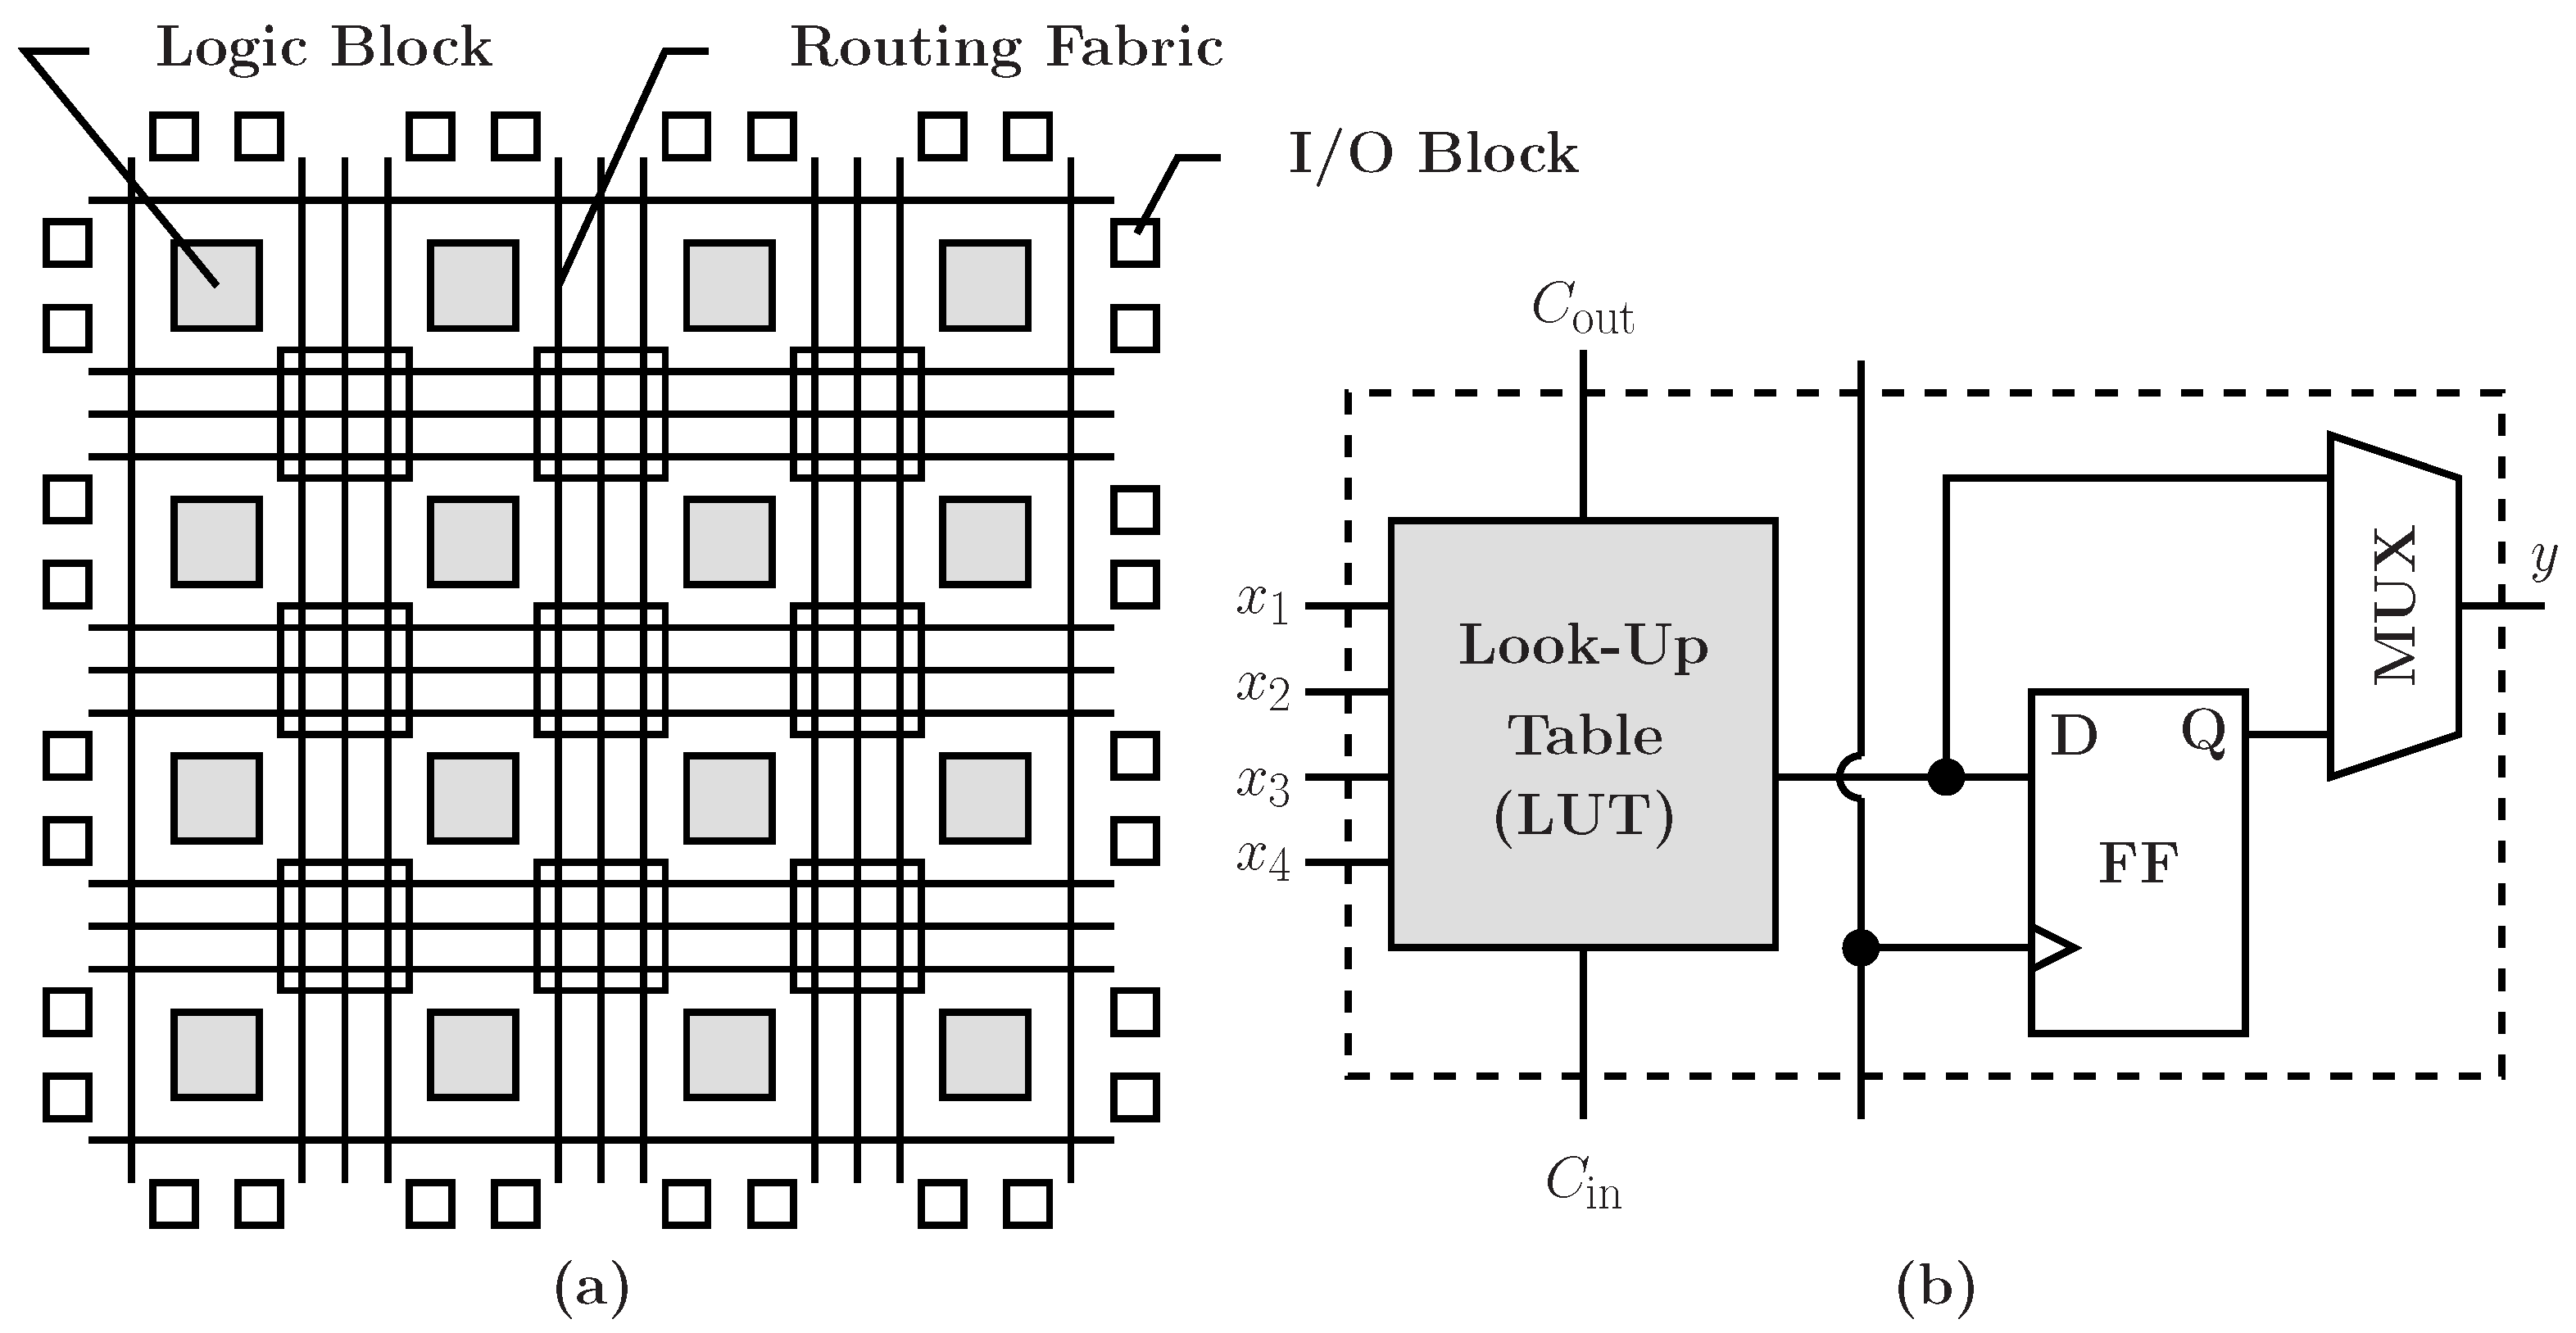
\includegraphics[]{fpga1}
	\caption{Schema FPGA}
\end{figure}

\section{Scrivere e compilare System Verilog}

Creiamo un multiplexer da due bit con System Verilog, compiliamo e visualizziamo con \textbf{GTKWave}

\includecode[verilog]{./verilog/2x1mux/mux.sv}{mux.sv}
\includecode[verilog]{./verilog/2x1mux/test_mux.sv}{test\_mux.sv}

Per compilare, eseguiamo da terminale 
\begin{lstlisting}[style={bash}]
iverilog -g2005-sv nome_sorgente.sv -o nome_eseguibile
\end{lstlisting}

Quindi, per compilare entrambi i file e caricarli in GTKWave:
\begin{lstlisting}[style={bash}]
iverilog -g2005-sv test_mux.sv mux.sv -o test_mux
# Eseguiamo la simulazione
./test_mux
# Viene creato il file provamux.vcd, carichiamolo in GTKWave
gtkwave provamux.vcd &
\end{lstlisting}

\includecode[verilog]{./verilog/2x1mux/mux4.sv}{Multiplexer da 4 vie ad 1 bit}

\includecode[verilog]{./verilog/2x1mux/muxbool.sv}{Multiplexer di variabili booleane}

\clearpage

\section{Esercizi}
\subsection{Automa che riconosce "abba"}

Realizziamo un automa di Mealy che riconosce le stringhe \textit{"abba"} da un insieme $ \{a,b,c\} $. La rete sequenziale dell'automa si realizzerà con i componenti visti in figura ~\ref{fig:mealyautomata1.tex}. Consideriamo la rappresentazione binaria dell'alfabeto con $ a = 00, b = 01, c = 11 $. Per gli stati usiamo la codifica $ S_1 = 00, S_2 = 01, S_3 = 11, S_4 = 10 $

\begin{figure}[H]
	\centering
	\caption{Automa di Mealy che riconosce "abba"}
	\begin{tikzpicture}[->,>=stealth',shorten >=1pt,auto,node distance=3.5cm]
	
	\node[state,accepting] 	(A)                    {$S_1$};
	\node[state]         	(B) [above right of=A] 	   {$S_2$};
	\node[state]         	(C) [below right of=B] 	   {$S_3$};
	\node[state]         	(D) [below right of=A] 	   {$S_4$};
	
	\path 	(A)		edge [bend left]  	node {$a/0$} 		(B)
	edge [loop left] 	node {$b,c/0$} 		(A)
	(B) 	edge [loop above] 	node {$a/0$} 		(B)
	edge [bend left] 	node {$c/0$} 		(A)
	edge [bend left]  	node {$b/0$} 		(C)
	(C)		edge [bend left]  	node {$c/0$} 		(A)
	edge [bend left]  	node {$a/0$} 		(B)
	edge [bend left]  	node {$b/0$} 		(D)
	(D)		edge [bend left]  	node {$b,c/0$} 		(A);
	\end{tikzpicture}
\end{figure}

\begin{table}[H]
	\centering
	\caption{Tabella di verità dell'output della rete sequenziale dell'automa "abba" ($ \omega $)}
	\label{tab:mealyomega2}
	\begin{tabular}{l|llll|l|}
		\cline{2-6}
		& $s_1$ & $s_2$ & $x_1$ & $x_2$ & z \\ \cline{2-6} 
		Stato $S_1$ & 0     & 0     & -     & -     & 0 \\
		Stato $S_2$ & 0     & 1     & -     & -     & 0 \\
		Stato $S_3$ & 1     & 1     & -     & -     & 0 \\
		Stato $S_4$ & 1     & 0     & 0     & 0     & 1 \\
		& 1     & 0     & 0     & 1     & 0 \\
		& 1     & 0     & 1     & 1     & 0 \\ \cline{2-6} 
	\end{tabular}
\end{table}

\begin{table}[H]
	\centering
	\caption{Tabella di verità del cambio di stato dell'automa per riconoscere "abba" ($\sigma$)}
	\label{tab:mealysigma2}
	\begin{tabular}{l|llll|ll|}
		\cline{2-7}
		& $s_1$ & $s_2$ & $x_1$ & $x_2$ & $s_1'$ & $s_2'$ \\ \cline{2-7} 
		Stato $S_1$ & 0     & 0     & 0     & 0     & 0      & 1      \\
		& 0     & 0     & 0     & 1     & 0      & 0      \\
		& 0     & 0     & 1     & 1     & 0      & 0      \\ \cline{2-7} 
		Stato $S_2$ & 0     & 1     & 0     & 0     & 0      & 1      \\
		& 0     & 1     & 0     & 1     & 1      & 1      \\
		& 0     & 1     & 1     & 1     & 0      & 0      \\ \cline{2-7} 
		Stato $S_3$ & 1     & 1     & 0     & 0     & 0      & 1      \\
		& 1     & 1     & 0     & 1     & 1      & 0      \\
		& 1     & 1     & 1     & 1     & 0      & 0      \\ \cline{2-7} 
		Stato $S_4$ & 1     & 0     & 0     & 0     & 0      & 0      \\
		& 1     & 0     & 0     & 1     & 0      & 0      \\
		& 1     & 0     & 1     & 1     & 0      & 0      \\ \cline{2-7} 
	\end{tabular}
\end{table}

% TODO mappa di karnaugh di s1 e s2

Avremo che la formula booleana sarà per il primo e secondo bit di stato:
\[ s_1' = \overbar{s_1}s_2\overbar{x_1}x_2 + s_1s_2\overbar{x_1}x_2 = s_2\overbar{x_1}x_2 \]. 
\[ s_2' = \overbar{s_1s_2}+ \overbar{s_1}s_2\overbar{x_1} + s_2\overbar{x_2}\]

La formula per l'uscita sarà $ z = s_1\overbar{s_2x_1x_2} $. Ci rimane da definire il registro da 2 bit per definire tutta la rete sequenziale. Abbiamo supposto che la rete sequenziale funzioni ricevendo un segnale di clock ad intervalli regolari.
La rete di output $ \omega $ è definita utilizzando soltanto AND ed impiegherà $ \Delta t $ per eseguire l'operazione. La funzione di cambio di stato $ \sigma $ è definita invece con 1 AND e 1 OR ed impiegherà $ 2\Delta t $ per l'operazione.
Il ciclo di clock dev'essere almeno $ \tau = \delta + \max\{t_{\sigma}, t_{\omega}\} $ dove $ \delta $ è la durata del segnale HIGH nel clock.

Abbiamo 3 moduli. Uno per il registro, uno per il modulo $ \omega $ e uno per il modulo $ \sigma $. Scriviamolo in Verilog.

\paragraph{Note}

La sintassi \verb|[a:b]| denota un array indicizzato dal numero \verb|a| al numero \verb|b|. Utilizziamo gli array per rappresentare valori a più bit. In questo caso, il registro è generalizzato per un parametro \verb|N| e può ad esempio essere inizializzato con \verb|registro #(4) nome(...) | dove 4 è il parametro \verb|N| e corrisponde al numero di bit del registro.

La negazione con \verb|!| nega un singolo valore, mentre la notazione \verb|~| viene detta negazione \textit{bit wise} e nega tutti i valori di una sequenza di bit.

Normalmente, in un blocco \verb|assign| assegno un valore ad una variabile booleana istantaneamente. Posso invece aggiungere un delay inserendo \verb|#x| di fronte all'identificatore della variabile, dove \verb|x| è un numero. Ad esempio:
\begin{lstlisting}[style={verilog}]
assign 
	#1 z = (ic == 0 ? x : y)
\end{lstlisting}

\includecode[verilog]{./verilog/abba/Registro/reg.v}{Registro a N bit}
\includecode[verilog]{./verilog/abba/Mealy/sigma.v}{Modulo di $ \sigma $ o funzione di cambio di stato}
\includecode[verilog]{./verilog/abba/Mealy/omega.v}{Modulo di $ \omega $}
\includecode[verilog]{./verilog/abba/Mealy/m1.v}{Modulo della rete sequenziale}
\includecode[verilog]{./verilog/abba/Mealy/test-m1.v}{Modulo di test della rete sequenziale}

\clearpage

\subsection{Automa di Moore per riconoscere "abba"}
Vediamo adesso un automa di Moore per riconoscere la stringa \textit{"abba"} nell'alfabeto $ \{a,b,c\} $. La differenza sta nel fatto che i singoli nodi non hanno accesso all'input $ x $.

\begin{figure}
	\centering
	\caption{Automa di Moore che riconosce "abba"}
	\begin{tikzpicture}[->,>=stealth',shorten >=1pt,auto,node distance=3.5cm]
	
	\node[state,initial] 	(A)                    {$\dfrac{S_1}{0}$};
	\node[state]         	(B) [right of=A] 	   {$\dfrac{S_2}{0}$};
	\node[state]         	(C) [below of=A] 	   {$\dfrac{S_3}{0}$};
	\node[state]         	(D) [below of=B] 	   {$\dfrac{S_4}{0}$};
	\node[state,accepting]  (E) [above right of=D] 	   {$\dfrac{S_4}{0}$};
	
	\path 	(A)		edge [bend left=60]  				node {$a$} 		(B)
					edge [loop above] 					node {$b,c$} 	(A)
			(B) 	edge [loop above] 					node {$a$} 		(B)
					edge [] 							node {$c$} 		(A)
					edge [bend left=20]  				node {$b$} 		(C)
			(C)		edge []  							node {$c$} 		(A)
					edge [bend left=20]  				node {$a$} 		(B)
					edge []  							node {$b$} 		(D)
			(D)		edge [bend left=90,looseness=2]		node {$b,c$} 	(A)
					edge []								node {$a$}		(E)
			(E)		edge [bend right=90,looseness=1.8]  	node {$b,c$} 	(A)
					edge []	node {$a$}		(B);
	\end{tikzpicture}
\end{figure}

\includecode[verilog]{./verilog/abba/Moore/mo-sigma.v}{Modulo di $ \sigma $ o funzione di cambio di stato (Moore)}
\includecode[verilog]{./verilog/abba/Moore/mo-omega.v}{Modulo di $ \omega $ (Moore)}
\includecode[verilog]{./verilog/abba/Moore/moore.v}{Modulo della rete sequenziale (Moore)}
\includecode[verilog]{./verilog/abba/Moore/test-m1.v}{Modulo di test della rete sequenziale (Moore)}
\includecode[makefile]{./verilog/abba/Moore/makefile}{Makefile (Moore)}

\FloatBarrier

\subsection{Mealy con Delay $ \equiv $ Moore}

\includecode[verilog]{./verilog/abba/MealyConDelay/reg-delay.v}{Registro a N bit con delay}
\includecode[verilog]{./verilog/abba/MealyConDelay/sigma-delay.v}{Modulo di $ \sigma $ o funzione di cambio di stato (Mealy con Delay)}
\includecode[verilog]{./verilog/abba/MealyConDelay/omega-delay.v}{Modulo di $ \omega $ (Mealy con Delay)}
\includecode[verilog]{./verilog/abba/MealyConDelay/m1-delay.v}{Modulo della rete sequenziale (Mealy con Delay)}
\includecode[verilog]{./verilog/abba/MealyConDelay/test-m1-delay.v}{Modulo di test della rete sequenziale (Mealy con Delay)}
\includecode[makefile]{./verilog/abba/MealyConDelay/makefile}{Makefile (Mealy con Delay)}

Per sincronizzare il modulo della rete sequenziale dell'automa di Mealy mettiamo un registro di fra l'input \verb|x| e le reti sequenziali \verb|sigma| e \verb|omega|


\backmatter
% bibliography, glossary and index would go here.

\end{document}